%!TEX root = ./template-skripsi.tex

\subsection{Sprint 9 Report}
Berikut merupakan report dari sprint ke-9 yang dilakukan pada tanggal 13 juli - 19 juli 2022.


\begin{longtable}{@{} |p{0.5cm}|p{5cm}|p{5cm}|p{2cm}| @{}}
\caption{Sprint-09 backlog.\label{table:sprint09_backlog}}\\

\hline
\textbf{No} & \textbf{\textit{Story}} & \textbf{\textit{Task}} & \textbf{\textit{Status}} \\
\hline
\endfirsthead

\hline
\endfoot

\hline
\multicolumn{4}{|c|}{Lanjutan Tabel \ref{table:sprint09_backlog}}\\
\hline
\textbf{No} & \textbf{\textit{Story}} & \textbf{\textit{Task}} & \textbf{\textit{Status}} \\
\hline
\endhead

		1 & \multirow{3}{5cm}{Create, Read, Updte, dan Delete untuk Pencatatan kualitas kolam harian dan mingguan} & Membarui desain database  & Completed\\
		\cline{1-1}\cline{3-4}
		2 & & Menambahkan routes API & Completed\\
		\cline{1-1}\cline{3-4}
		3 & & Implementasi controller entry Pencatatan kualitas kolam harian & Completed\\
		\cline{1-1}\cline{3-4}
		4 & & Implementasi controller fetch list Pencatatan kualitas kolam harian & Completed\\
		\cline{1-1}\cline{3-4}
		5 & & Implementasi controller edit Pencatatan kualitas kolam harian & Completed\\
		\cline{1-1}\cline{3-4}
		6 & & Implementasi controller delete Pencatatan kualitas kolam harian & Completed\\
		\cline{1-1}\cline{3-4}
		7 & & Implementasi controller fetch detail Pencatatan kualitas kolam harian dengan id& Completed\\
		\cline{1-1}\cline{3-4}
        		8 & & Implementasi controller entry Pencatatan kualitas kolam mingguan & Completed\\
		\cline{1-1}\cline{3-4}
		9 & & Implementasi controller fetch list Pencatatan kualitas kolam mingguan & Completed\\
		\cline{1-1}\cline{3-4}
		10 & & Implementasi controller edit Pencatatan kualitas kolam mingguan & Completed\\
		\cline{1-1}\cline{3-4}
		11 & & Implementasi controller delete Pencatatan kualitas kolam mingguan & Completed\\
		\cline{1-1}\cline{3-4}
		12 & & Implementasi controller fetch detail Pencatatan kualitas kolam mingguan dengan id& Completed\\
		\cline{1-1}\cline{3-4}
		13 & & Membuat view rekap Pencatatan kualitas kolam harian & Completed\\
		\cline{1-1}\cline{3-4}
		14 & & Membuat view rekap Pencatatan kualitas kolam mingguan & Completed\\
		\cline{1-1}\cline{3-4}
		\hline

\end{longtable}

\begin{enumerate}[1.]

\item \textbf{Membarui desain database}

\begin{figure}[H]
	\centering
	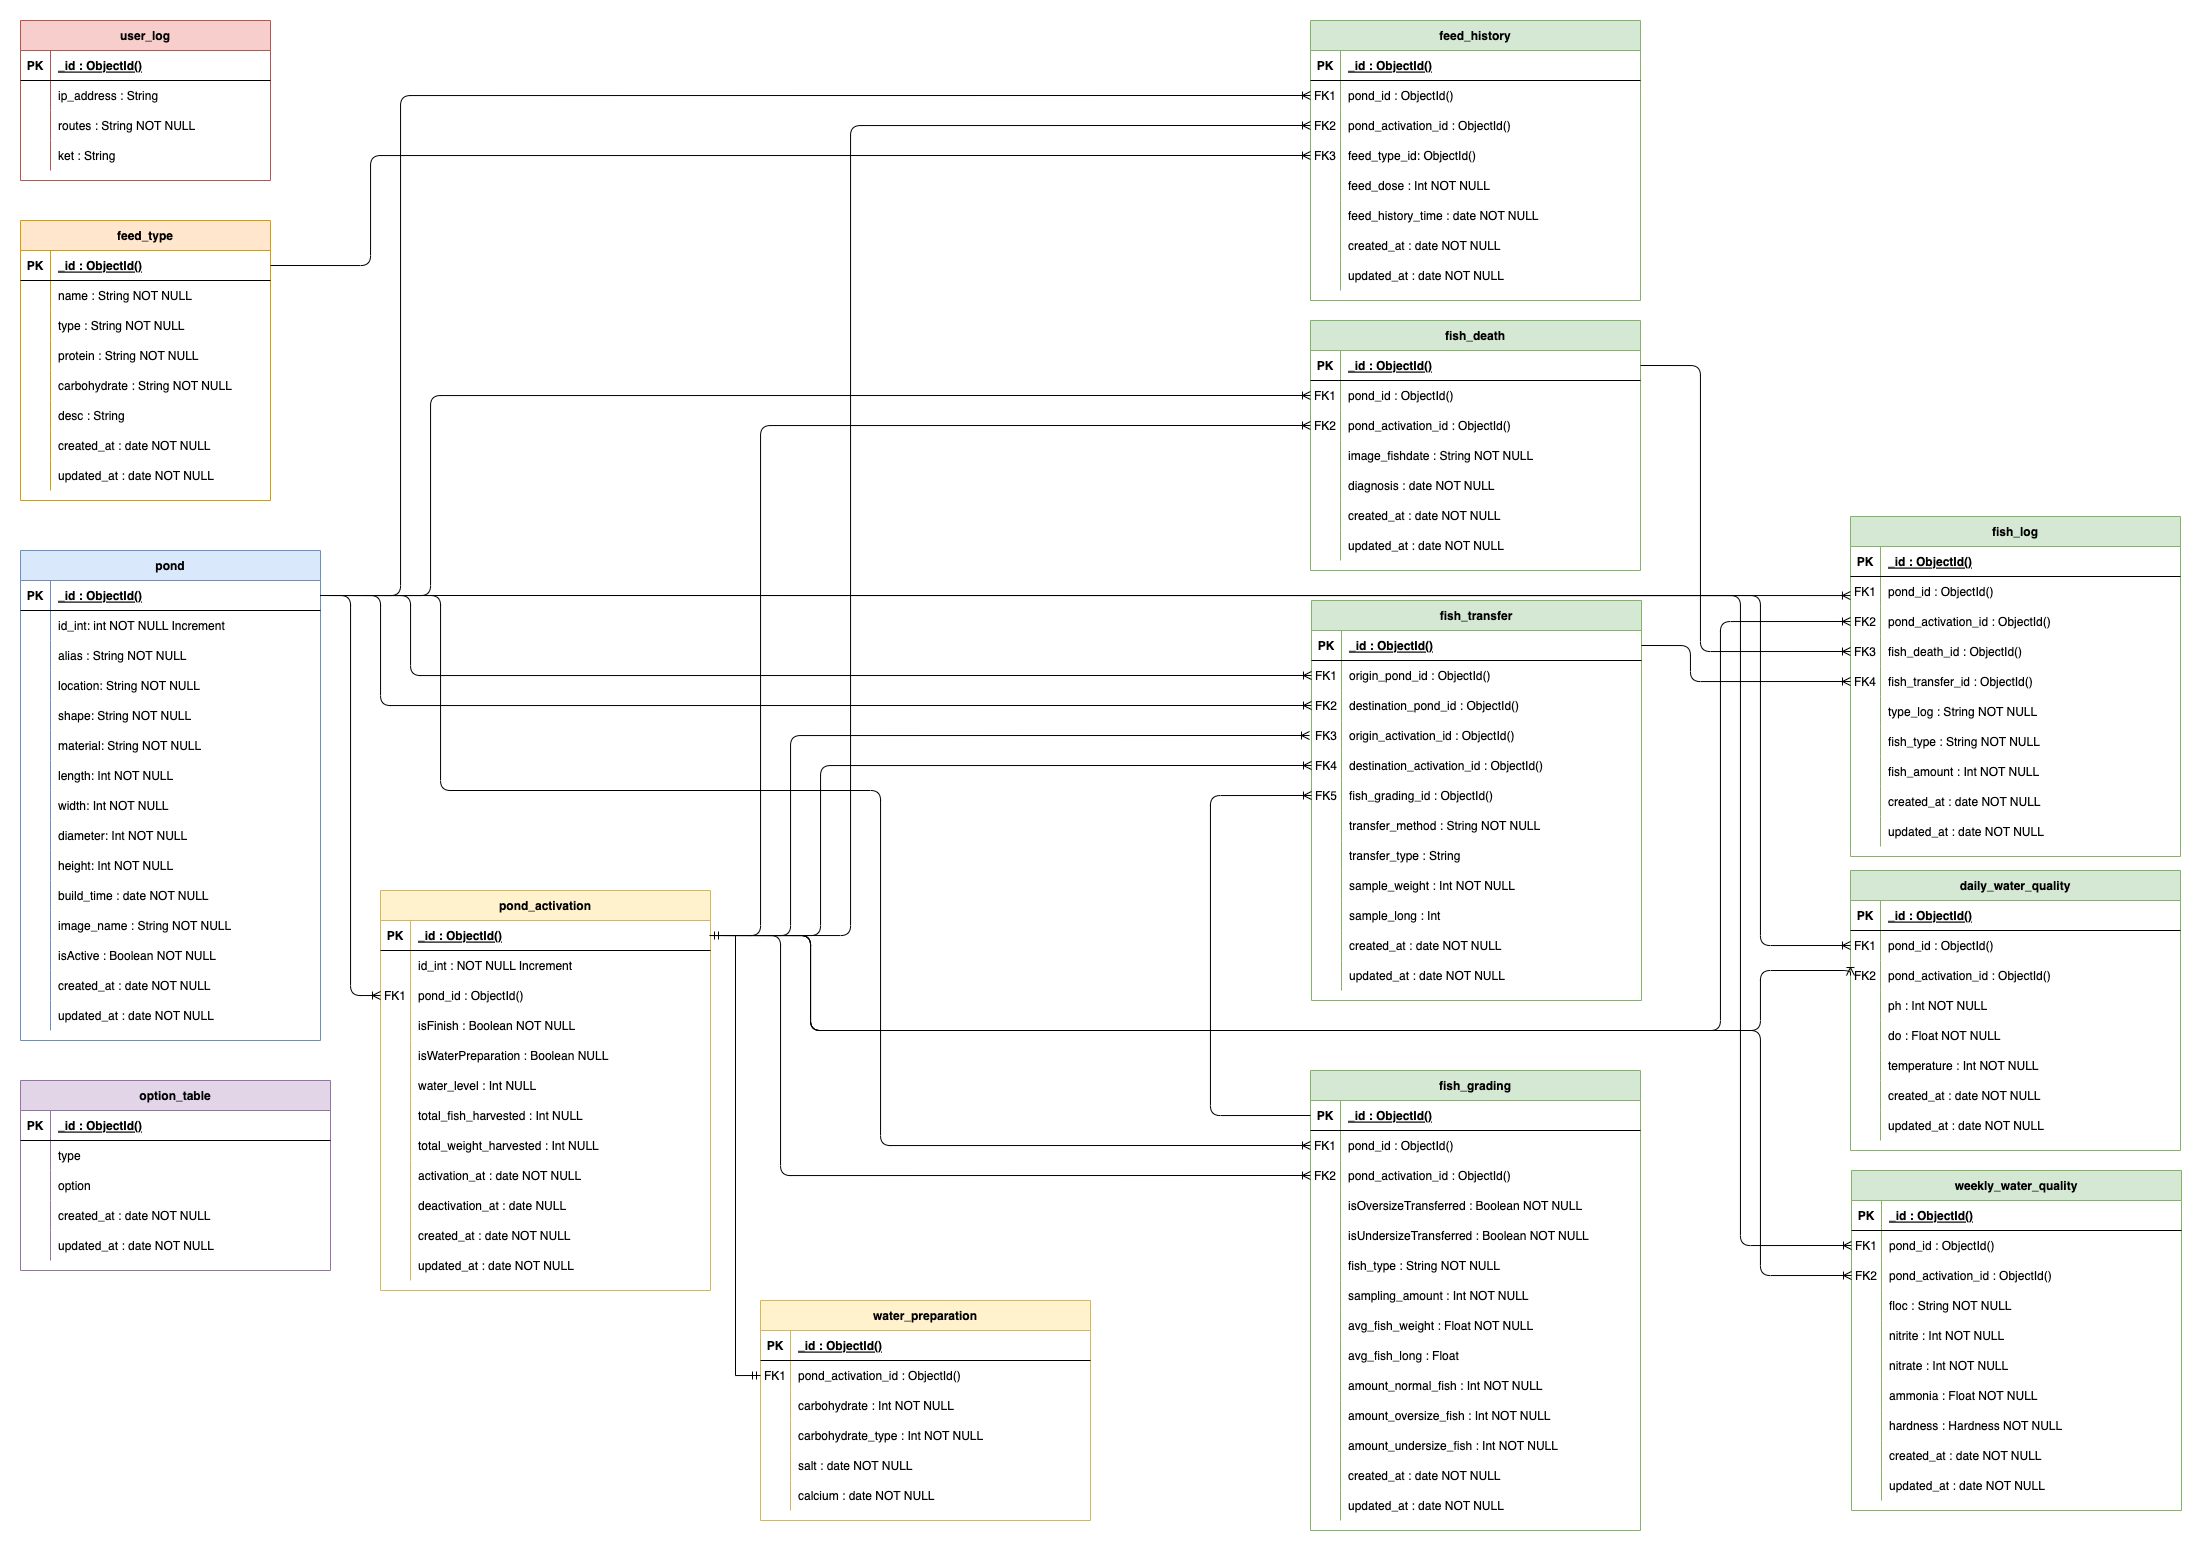
\includegraphics[height=0.7\textwidth]{gambar/Sprint09/diagram database/database}
	\caption{ERD Database Sprint-9}
	\label{fig:database_sprint9}
\end{figure}

Dengan berubahnya desain database diperlukan juga penambahan model pada source code, berikut perubahan pada source code model.

\begin{lstlisting}
# fishapi/database/model.py

class DailyWaterQuality(db.Document):
    pond_id = db.ReferenceField(Pond, required=True)
    pond_activation_id = db.ReferenceField(PondActivation, required=True)
    ph = db.IntField(required=True)
    do = db.FloatField(required=True)
    temperature = db.IntField(required=True)
    created_at = db.DateTimeField(default=datetime.datetime.now)
    updated_at = db.DateTimeField(default=datetime.datetime.now)


class WeeklyWaterQuality(db.Document):
    floc_option = ('0-10', '11-30', '31-50', '51-100', '101-300', '>300')
    nitrite_option = (0, 1, 5, 10, 20, 40, 80)
    nitrate_option = (0, 10, 25, 50, 100, 250, 500)
    ammonia_option = (0, 0.25, 1.5, 3, 5)
    hardness_option = (0, 25, 50, 125, 250, 425)

    pond_id = db.ReferenceField(Pond, required=True)
    pond_activation_id = db.ReferenceField(PondActivation, required=True)
    floc = db.StringField(required=True, choices=floc_option)
    nitrite = db.IntField(required=True, choices=nitrite_option)
    nitrate = db.IntField(required=True, choices=nitrate_option)
    ammonia = db.FloatField(required=True, choices=ammonia_option)
    hardness = db.IntField(required=True, choices=hardness_option)
    created_at = db.DateTimeField(default=datetime.datetime.now)
    updated_at = db.DateTimeField(default=datetime.datetime.now)
\end{lstlisting}



\item \textbf{Menambahkan routes API}

\begin{lstlisting}
# fishapi/resource/routes.py

# daily water
    api.add_resource(DailyWaterQualitysApi, '/api/dailywaterquality')
    api.add_resource(DailyWaterQualityApi, '/api/dailywaterquality/<id>')

    # weekly water
    api.add_resource(WeeklyWaterQualitysApi, '/api/weeklywaterquality')
    api.add_resource(WeeklyWaterQualityApi, '/api/weeklywaterquality/<id>')
\end{lstlisting}




\item \textbf{Implementasi controller entry pencatatan kualitas kolam harian}

Implementasi controller API entry pencatatan kualitas kolam harian, berikut merupakan perubahan source code controller API entry pencatatan kualitas kolam harian.

\begin{lstlisting}
# fishapi/resource/dailywaterquality.py

class DailyWaterQualitysApi(Resource):
    def post(self):
        try:
            pond_id = request.form.get("pond_id", None)
            pond = Pond.objects.get(id=pond_id)
            if pond['isActive'] == False:
                response = {"message": "pond is not active"}
                response = json.dumps(response, default=str)
                return Response(response, mimetype="application/json", status=400)
            pond_activation = PondActivation.objects(
                pond_id=pond_id, isFinish=False).order_by('-activated_at').first()
            body = {
                "pond_id": pond.id,
                "pond_activation_id": pond_activation.id,
                "ph": request.form.get("ph", None),
                "do": request.form.get("do", None),
                "temperature": request.form.get("temperature", None),
            }
            print(body)
            dailywaterquality = DailyWaterQuality(**body).save()
            id = dailywaterquality.id
            response = {
                "message": "success add data daily water quality", "id": id}
            response = json.dumps(response, default=str)
            return Response(response, mimetype="application/json", status=200)
        except Exception as e:
            response = {"message": str(e)}
            response = json.dumps(response, default=str)
            return Response(response, mimetype="application/json", status=400)
\end{lstlisting}


Kode di atas merupakan implementasi sebuah API endpoint dengan kelas DailyWaterQualitysApi. Kode tersebut berfungsi untuk menangani permintaan HTTP POST yang diterima pada endpoint tersebut. Berikut adalah penjelasan langkah-langkah yang dilakukan oleh kode tersebut:

\begin{enumerate}
\item Metode post() digunakan untuk menangani permintaan POST pada endpoint DailyWaterQualitysApi.
\item Di dalam blok try, pertama-tama dilakukan pengambilan nilai pond\_id dari data form yang dikirim dalam permintaan.
\item Kemudian, dilakukan pencarian objek Pond berdasarkan pond\_id yang diperoleh.
\item Jika nilai isActive pada objek Pond adalah False, artinya kolam tidak aktif, maka akan mengembalikan respons dengan pesan error yang sesuai.
\item Selanjutnya, dilakukan pencarian objek PondActivation terbaru (dengan isFinish bernilai False) berdasarkan pond\_id yang diperoleh, dengan urutan berdasarkan activated\_at secara menurun.
\item Data yang diperoleh dari form dan informasi kolam dan aktivasi yang ditemukan digabungkan ke dalam variabel body.
\item Objek DailyWaterQuality baru dibuat dengan menggunakan nilai-nilai dari body dan kemudian disimpan ke database dengan menggunakan metode .save(). Hasilnya akan disimpan dalam variabel dailywaterquality.
\item Dari objek dailywaterquality, diambil nilai id dan disimpan dalam variabel id.
\item Hasil akhir yang akan dikembalikan sebagai respons adalah pesan sukses beserta id dari data yang berhasil ditambahkan dalam format JSON.
\item Jika terjadi exception atau kesalahan, akan di-handle dengan mengembalikan respons dengan pesan error yang sesuai dalam format JSON dan status kode 400.
\end{enumerate}
Dengan demikian, kode tersebut mengimplementasikan logika untuk menambahkan data kualitas air harian (DailyWaterQuality) ke dalam database berdasarkan permintaan POST yang diterima.

Berikut merupakan form untuk entry pencatatan kualitas kolam harian.

\begin{longtable}{| l | p{5cm} | p{5cm} |}
\caption{Form entry pencatatan kolam harian.\label{table:form_entry_pencatatan_kolam_harian}}\\

\hline
\multicolumn{1}{|c|}{\textbf{Form}} & \multicolumn{1}{|c|}{\textbf{Jenis Data}} & \multicolumn{1}{|c|}{\textbf{Deskripsi}}\\
\hline
\endfirsthead

\hline
\multicolumn{3}{|c|}{Lanjutan Tabel \ref{table:form_entry_pencatatan_kolam_harian}}\\
\hline
\multicolumn{1}{|c|}{\textbf{Form}} & \multicolumn{1}{|c|}{\textbf{Jenis Data}} & \multicolumn{1}{|c|}{\textbf{Deskripsi}}\\
\hline
\endhead

                                          

pond\_id   & REQUIRED STRING & id kolam yang akan di lakukan pencatatan kualitas air harian \\ \hline
ph         & REQUIRED INT    & tingkat ph air satuan (pH)                                   \\ \hline
do         & REQUIRED INT    & oksigen yang terlarut dalam air (ppm)                        \\ \hline
temprature & REQUIRED INT    & suhu air kolam (\textdegree C)                \\ \hline
\end{longtable}



Tabel di atas menggambarkan struktur data yang diperlukan untuk melakukan pencatatan kualitas air harian dalam kolam. Berikut adalah penjelasan untuk setiap kolom dalam tabel:

\begin{enumerate}

\item pond\_id: Kolom ini merupakan string yang wajib diisi. Nilai yang dimasukkan adalah ID kolam yang akan dicatat kualitas air hariannya. Kolom ini digunakan untuk mengaitkan catatan kualitas air dengan kolam yang sesuai.

\item ph: Kolom ini merupakan integer yang wajib diisi. Nilai yang dimasukkan adalah tingkat pH air dalam satuan pH (potensi hidrogen). pH mengindikasikan tingkat keasaman atau kebasaan air. Pengukuran ini penting karena kualitas air yang baik untuk ikan seringkali terkait dengan tingkat pH yang sesuai.

\item do: Kolom ini merupakan integer yang wajib diisi. Nilai yang dimasukkan adalah tingkat oksigen terlarut dalam air dalam satuan ppm (parts per million). Oksigen terlarut penting untuk kelangsungan hidup ikan dan organisme akuatik lainnya. Pemantauan kadar oksigen terlarut membantu memastikan bahwa lingkungan air di dalam kolam memadai bagi ikan.

\item temperature: Kolom ini merupakan integer yang wajib diisi. Nilai yang dimasukkan adalah suhu air kolam dalam satuan derajat Celsius. Suhu air mempengaruhi kesehatan dan pertumbuhan ikan. Pengukuran suhu air membantu memantau perubahan suhu yang dapat memengaruhi kondisi ikan dan keseimbangan ekosistem di dalam kolam.

\end{enumerate}

Dengan menggunakan struktur data yang terdefinisi dalam tabel ini, pengguna dapat mencatat kualitas air harian dengan mengisi nilai-nilai yang sesuai untuk setiap kolom. Data ini penting untuk pemantauan dan pengelolaan yang efektif dalam budidaya ikan, serta untuk menjaga kesehatan dan kualitas lingkungan air di dalam kolam.


Berikut merupakan hasil test request dari API entry pencatatan kolam harian.

cURL:

\begin{lstlisting}
curl --location 'http://jft.web.id/fishapi/api/dailywaterquality' \
--form 'pond_id="{pond_id}"' \
--form 'ph="1"' \
--form 'do="6"' \
--form 'temperature="20"'
\end{lstlisting}

response json:

\begin{lstlisting}
{
  "message": "success add data daily water quality",
  "id": "62e8b800ef4edacc5bb18b05"
}
\end{lstlisting}




\item \textbf{Implementasi API fetch list pencatatan kolam harian}

Implementasi controller API fetch list pencatatan kolam harian, berikut merupakan source code controller API fetch list pencatatan kolam harian.

\begin{lstlisting}
# fishapi/resource/dailywaterquality.py

class DailyWaterQualitysApi(Resource):
    def get(self):
        try:
            pipeline = [
                {"$sort": {"created_at": -1}},
                {'$lookup': {
                    'from': 'pond',
                    'let': {"pondid": "$pond_id"},
                    'pipeline': [
                        {'$match': {'$expr': {'$eq': ['$_id', '$$pondid']}}},
                        {"$project": {
                            "_id": 1,
                            "alias": 1,
                            "location": 1,
                            "build_at": 1,
                            "isActive": 1,
                        }}
                    ],
                    'as': 'pond'
                }},
                {'$lookup': {
                    'from': 'pond_activation',
                    'let': {"activationid": "$pond_activation_id"},
                    'pipeline': [
                        {'$match': {
                            '$expr': {'$eq': ['$_id', '$$activationid']}}},
                        {"$project": {
                            "_id": 1,
                            "isFinish": 1,
                            "isWaterPreparation": 1,
                            "water_level": 1,
                            "activated_at": 1
                        }}
                    ],
                    'as': 'pond_activation'
                }},
                {"$addFields": {
                    "pond": {"$first": "$pond"},
                    "pond_activation": {"$first": "$pond_activation"},
                    "ph_desc": {
                        "$switch":
                            {
                                "branches": [
                                    {
                                        "case": {"$lt": ["$ph", 6]},
                                        "then": "berbahaya"
                                    },
                                    {
                                        "case": {"$gt": ["$ph", 8]},
                                        "then": "berbahaya"
                                    }
                                ],
                                "default": "normal"
                            }
                    },
                    "do_desc": {
                        "$switch":
                            {
                                "branches": [
                                    {
                                        "case": {"$or": [
                                            {"$lt": ["$do", 3]},
                                            {"$gt": ["$do", 7.5]}
                                        ]},
                                        "then": "berbahaya"
                                    },
                                    {
                                        "case": {"$or": [
                                            {"$and": [{"$gte": ["$do", 3]}, {
                                                "$lte": ["$do", 4]}]},
                                            {"$and": [{"$gt": ["$do", 6]}, {
                                                "$lte": ["$do", 7.5]}]}
                                        ]},
                                        "then": "semi berbahaya"
                                    }
                                ],
                                "default": "normal"
                            }
                    }
                }},
                {"$project": {
                    "updated_at": 0,
                    "created_at": 0,
                }}
            ]
            dailywaterquality = DailyWaterQuality.objects.aggregate(pipeline)
            list_dailywaterqualitys = list(dailywaterquality)
            response = json.dumps(list_dailywaterqualitys, default=str)
            return Response(response, mimetype="application/json", status=200)
        except Exception as e:
            response = {"message": str(e)}
            response = json.dumps(response, default=str)
            return Response(response, mimetype="application/json", status=400)
\end{lstlisting}


Kode di atas merupakan implementasi dari sebuah API dengan nama DailyWaterQualitysApi yang bertujuan untuk mengambil data kualitas air harian (DailyWaterQuality). Berikut penjelasan tentang kode tersebut:

API ini menyediakan metode get() yang digunakan untuk mengambil data kualitas air harian. Dalam metode tersebut, dilakukan serangkaian operasi pengolahan data menggunakan Aggregation Framework pada MongoDB.

Pertama, sebuah pipeline dibuat sebagai langkah-langkah pengolahan data. Pada langkah awal, data diurutkan berdasarkan waktu pembuatan (created\_at) secara menurun (descending) menggunakan operasi \$sort.

Selanjutnya, dilakukan operasi \$lookup untuk melakukan join dengan dua koleksi lain, yaitu "pond" dan "pond\_activation". Dalam langkah ini, dilakukan pencocokan (\$match) berdasarkan nilai \_id pada koleksi "pond" dan "pond\_activation" dengan nilai yang berasal dari koleksi "DailyWaterQuality". Hasil join disimpan dalam array pond dan pond\_activation.

Setelah itu, dilakukan penambahan kolom baru (\$addFields) pada dokumen dengan menggunakan hasil join sebelumnya. Kolom baru yang ditambahkan antara lain pond (berisi data kolam yang terkait), pond\_activation (berisi data aktivasi kolam yang terkait), ph\_desc (deskripsi tingkat pH), dan do\_desc (deskripsi tingkat oksigen terlarut). Deskripsi tersebut ditentukan berdasarkan kondisi yang didefinisikan dengan operator \$switch.

Langkah terakhir dalam pipeline adalah menggunakan operasi \$project untuk menghilangkan kolom updated\_at dan created\_at dari hasil akhir.

Setelah pipeline selesai, dilakukan agregasi pada koleksi "DailyWaterQuality" menggunakan pipeline yang telah dibuat. Hasil agregasi kemudian diubah menjadi list dan dikonversi menjadi format JSON. Respon JSON ini kemudian dikembalikan sebagai respons dari API dengan kode status 200 (OK).

Namun, jika terjadi kesalahan selama proses, dilakukan penanganan eksepsi (exception) yang menghasilkan pesan error. Pesan error tersebut kemudian dikonversi menjadi format JSON dan dikembalikan sebagai respons dari API dengan kode status 400 (Bad Request).

Berikut merupakan hasil test request dari API fetch list pencatatan kolam harian.

cURL:

\begin{lstlisting}
curl --location 'http://jft.web.id/fishapi/api/dailywaterquality'
\end{lstlisting}

response json:

\begin{lstlisting}
[
    {
        "_id": "647edbe028aa8efac0b6c2f2",
        "pond_id": "647d8beb28aa8efac0b6c2ed",
        "pond_activation_id": "647d8c0b28aa8efac0b6c2ee",
        "ph": 1,
        "do": 6.0,
        "temperature": 20,
        "pond": {
            "_id": "647d8beb28aa8efac0b6c2ed",
            "alias": "charlie",
            "location": "blok 3",
            "isActive": true,
            "build_at": "2023-06-05 14:16:59.384000"
        },
        "pond_activation": {
            "_id": "647d8c0b28aa8efac0b6c2ee",
            "isFinish": false,
            "isWaterPreparation": false,
            "water_level": 100.0,
            "activated_at": "2023-06-05 14:17:31.973000"
        },
        "ph_desc": "berbahaya",
        "do_desc": "normal"
    },
    {
        "_id": "647edbe028aa8efac0b6c2f2",
        "pond_id": "647d8beb28aa8efac0b6c2ed",
        "pond_activation_id": "647d8c0b28aa8efac0b6c2ee",
        "ph": 1,
        "do": 6.0,
        "temperature": 20,
        "pond": {
            "_id": "647d8beb28aa8efac0b6c2ed",
            "alias": "charlie",
            "location": "blok 3",
            "isActive": true,
            "build_at": "2023-06-05 14:16:59.384000"
        },
        "pond_activation": {
            "_id": "647d8c0b28aa8efac0b6c2ee",
            "isFinish": false,
            "isWaterPreparation": false,
            "water_level": 100.0,
            "activated_at": "2023-06-05 14:17:31.973000"
        },
        "ph_desc": "berbahaya",
        "do_desc": "normal"
    }
]
\end{lstlisting}



\item \textbf{Implementasi API edit pencatatan kolam harian}

Implementasi controller API edit pencatatan kolam harian, berikut merupakan perubahan source code controller API edit pencatatan kolam harian.

\begin{lstlisting}
# fishapi/database/dailywaterquality.py

class DailyWaterQualityApi(Resource):
    def put(self, id):
        try:
            body = request.form.to_dict(flat=True)
            DailyWaterQuality.objects.get(id=id).update(**body)
            response = {
                "message": "success change data daily water quality", "id": id}
            response = json.dumps(response, default=str)
            return Response(response, mimetype="application/json", status=200)
        except Exception as e:
            response = {"message": str(e)}
            response = json.dumps(response, default=str)
            return Response(response, mimetype="application/json", status=400)
\end{lstlisting}

Kode di atas merupakan implementasi dari sebuah API dengan nama DailyWaterQualityApi yang bertujuan untuk mengubah (update) data kualitas air harian (DailyWaterQuality) berdasarkan ID tertentu. Berikut adalah penjelasan tentang kode tersebut:

API ini menyediakan metode put() yang digunakan untuk mengubah data kualitas air harian. Metode ini menerima parameter id yang merupakan ID dari data yang akan diubah.

Dalam metode put(), terdapat beberapa langkah yang dilakukan. Pertama, nilai dari form request diubah menjadi bentuk dictionary menggunakan fungsi request.form.to\_dict(flat=True). Dictionary ini akan berisi data yang dikirimkan dalam form request.

Selanjutnya, dilakukan operasi update() pada objek DailyWaterQuality dengan menggunakan ID yang diberikan. Operasi update() ini akan memperbarui data dengan nilai-nilai yang terdapat dalam dictionary body. Data yang diubah akan sesuai dengan kolom-kolom yang ada dalam objek DailyWaterQuality.

Setelah proses pembaruan selesai, dibuat respons yang akan dikirimkan kembali kepada pengguna. Respons ini berupa pesan sukses yang mengindikasikan bahwa data kualitas air harian telah berhasil diubah. Respons tersebut juga mencakup ID dari data yang telah diubah. Pesan dan ID tersebut kemudian diubah menjadi format JSON menggunakan fungsi json.dumps().

Apabila terjadi kesalahan selama proses pembaruan, penanganan eksepsi (exception handling) akan terjadi. Pesan error yang dihasilkan akan dikonversi menjadi format JSON dan dikirimkan sebagai respons dengan kode status 400 (Bad Request).

Dengan demikian, melalui API ini pengguna dapat mengirimkan permintaan untuk mengubah data kualitas air harian berdasarkan ID tertentu, dan akan menerima respons yang mengindikasikan keberhasilan atau kegagalan pembaruan data.

Berikut merupakan hasil test request dari API edit pencatatan kolam harian.

cURL:

\begin{lstlisting}
curl --location --request PUT 'http://jft.web.id/fishapi/api/dailywaterquality/62e89ce7846724c2d2984687' \
--form 'ph="2"' \
--form 'do="7"' \
--form 'temperature="20"'
\end{lstlisting}

response json:

\begin{lstlisting}
{
  "message": "success change data daily water quality",
  "id": "62e89ce7846724c2d2984687"
}
\end{lstlisting}



\item \textbf{Implementasi API delete pencatatan kolam harian}

Implementasi controller API delete pencatatan kolam harian, berikut merupakan perubahan source code controller API delete pencatatan kolam harian.

\begin{lstlisting}
# fishapi/database/dailywaterquality.py

class DailyWaterQualityApi(Resource):
    def delete(self, id):
        try:
            dailywaterquality = DailyWaterQuality.objects.get(id=id).delete()
            response = {"message": "success delete daily water quality"}
            response = json.dumps(response, default=str)
            return Response(response, mimetype="application/json", status=200)
        except Exception as e:
            response = {"message": str(e)}
            response = json.dumps(response, default=str)
            return Response(response, mimetype="application/json", status=400)
\end{lstlisting}


API ini menyediakan metode delete() yang digunakan untuk menghapus data kualitas air harian. Metode ini menerima parameter id yang merupakan ID dari data yang akan dihapus.

Dalam metode delete(), terdapat beberapa langkah yang dilakukan. Pertama, dilakukan pengambilan objek DailyWaterQuality berdasarkan ID yang diberikan menggunakan metode get(). Kemudian, dilakukan operasi delete() pada objek tersebut untuk menghapus data dari koleksi.

Setelah proses penghapusan selesai, dibuat respons yang akan dikirimkan kembali kepada pengguna. Respons ini berupa pesan sukses yang mengindikasikan bahwa data kualitas air harian telah berhasil dihapus. Pesan tersebut kemudian diubah menjadi format JSON menggunakan fungsi json.dumps().

Apabila terjadi kesalahan selama proses penghapusan, penanganan eksepsi (exception handling) akan terjadi. Pesan error yang dihasilkan akan dikonversi menjadi format JSON dan dikirimkan sebagai respons dengan kode status 400 (Bad Request).

Dengan demikian, melalui API ini pengguna dapat mengirimkan permintaan untuk menghapus data kualitas air harian berdasarkan ID tertentu, dan akan menerima respons yang mengindikasikan keberhasilan atau kegagalan penghapusan data.

Berikut merupakan hasil test request dari API delete pencatatan kolam harian.

cURL:

\begin{lstlisting}
curl --location --request DELETE 'http://jft.web.id/fishapi/api/dailywaterquality/62e8b800ef4edacc5bb18b05'
\end{lstlisting}

response json:

\begin{lstlisting}
{
  "message": "success delete daily water quality"
}
\end{lstlisting}


\item \textbf{Implementasi API fetch detail pencatatan kolam harian dengan id}

Implementasi controller API fetch detail pencatatan kolam harian, berikut merupakan source code controller API fetch detail pencatatan kolam harian.

\begin{lstlisting}
# fishapi/resource/dailywaterquality.py

class DailyWaterQualityApi(Resource):
    def get(self, id):
        try:
            pipeline = [
                {'$match': {'$expr': {'$eq': ['$_id', {'$toObjectId': id}]}}},
                {'$lookup': {
                    'from': 'pond',
                    'let': {"pondid": "$pond_id"},
                    'pipeline': [
                        {'$match': {'$expr': {'$eq': ['$_id', '$$pondid']}}},
                        {"$project": {
                            "_id": 1,
                            "alias": 1,
                            "location": 1,
                            "build_at": 1,
                            "isActive": 1,
                        }}
                    ],
                    'as': 'pond'
                }},
                {'$lookup': {
                    'from': 'pond_activation',
                    'let': {"activationid": "$pond_activation_id"},
                    'pipeline': [
                        {'$match': {
                            '$expr': {'$eq': ['$_id', '$$activationid']}}},
                        {"$project": {
                            "_id": 1,
                            "isFinish": 1,
                            "isWaterPreparation": 1,
                            "water_level": 1,
                            "activated_at": 1
                        }}
                    ],
                    'as': 'pond_activation'
                }},
                {"$addFields": {
                    "pond": {"$first": "$pond"},
                    "pond_activation": {"$first": "$pond_activation"},
                    "ph_desc": {
                        "$switch":
                            {
                                "branches": [
                                    {
                                        "case": {"$lt": ["$ph", 6]},
                                        "then": "berbahaya"
                                    },
                                    {
                                        "case": {"$gt": ["$ph", 8]},
                                        "then": "berbahaya"
                                    }
                                ],
                                "default": "normal"
                            }
                    },
                    "do_desc": {
                        "$switch":
                            {
                                "branches": [
                                    {
                                        "case": {"$or": [
                                            {"$lt": ["$do", 3]},
                                            {"$gt": ["$do", 7.5]}
                                        ]},
                                        "then": "berbahaya"
                                    },
                                    {
                                        "case": {"$or": [
                                            {"$and": [{"$gte": ["$do", 3]}, {
                                                "$lte": ["$do", 4]}]},
                                            {"$and": [{"$gt": ["$do", 6]}, {
                                                "$lte": ["$do", 7.5]}]}
                                        ]},
                                        "then": "semi berbahaya"
                                    }
                                ],
                                "default": "normal"
                            }
                    }
                }},
                {"$project": {
                    "updated_at": 0,
                    "created_at": 0,
                }}
            ]
            dailywaterquality = DailyWaterQuality.objects.aggregate(pipeline)
            list_dailywaterqualitys = list(dailywaterquality)
            response = json.dumps(list_dailywaterqualitys[0], default=str)
            return Response(response, mimetype="application/json", status=200)
        except Exception as e:
            response = {"message": str(e)}
            response = json.dumps(response, default=str)
            return Response(response, mimetype="application/json", status=400)
\end{lstlisting}


Kode di atas merupakan implementasi dari sebuah API dengan nama DailyWaterQualityApi yang digunakan untuk mendapatkan (get) data kualitas air harian (DailyWaterQuality) berdasarkan ID tertentu. Berikut adalah penjelasan tentang kode tersebut:

API ini menyediakan metode get() yang digunakan untuk mengambil data kualitas air harian berdasarkan ID. Metode ini menerima parameter id yang merupakan ID dari data yang akan diambil.

Dalam metode get(), terdapat beberapa langkah yang dilakukan. Pertama, terdapat penggunaan pipeline yang berisi serangkaian tahapan untuk melakukan agregasi dan pencarian data menggunakan MongoDB. Tahapan-tahapan tersebut meliputi pencocokan (\$match) berdasarkan ID yang diberikan, pencarian relasi dengan koleksi pond dan pond\_activation menggunakan \$lookup, dan penambahan (\$addFields) beberapa field baru ke hasil agregasi.

Beberapa field baru yang ditambahkan adalah ph\_desc dan do\_desc, yang bergantung pada nilai ph dan do pada data kualitas air harian. Nilai-nilai tersebut diuji menggunakan operator \$switch untuk menentukan deskripsi kualitas air berdasarkan batasan-batasan tertentu.

Setelah tahapan agregasi selesai, hasil aggregasi tersebut dikonversi menjadi daftar (list) dan diambil elemen pertama (list\_dailywaterqualitys[0]). Hasil tersebut kemudian diubah menjadi format JSON menggunakan fungsi json.dumps().

Apabila terjadi kesalahan selama proses pengambilan data, penanganan eksepsi (exception handling) akan terjadi. Pesan error yang dihasilkan akan dikonversi menjadi format JSON dan dikirimkan sebagai respons dengan kode status 400 (Bad Request).


Berikut merupakan hasil test request dari API fetch pencatatan kolam harian berdasarkan id.

cURL:

\begin{lstlisting}
curl --location 'http://jft.web.id/fishapi/api/dailywaterquality/62e89ce7846724c2d2984687'
\end{lstlisting}

response json:

\begin{lstlisting}
{
  "_id": "62e89ce7846724c2d2984687",
  "pond_id": "62a62163e445ffb9c5f746f3",
  "pond_activation_id": "62d3f2180d7265ab60f9cb83",
  "ph": 7,
  "do": 4,
  "temperature": 25,
  "pond": {
    "_id": "62a62163e445ffb9c5f746f3",
    "alias": "charlie",
    "location": "blok 2",
    "build_at": "2022-06-13 00:24:51.473000",
    "isActive": true
  },
  "pond_activation": {
    "_id": "62d3f2180d7265ab60f9cb83",
    "isFinish": false,
    "isWaterPreparation": true,
    "water_level": 100,
    "activated_at": "2022-07-17 18:27:20.511000"
  },
  "ph_desc": "normal",
  "do_desc": "semi berbahaya"
}
\end{lstlisting}




\item \textbf{Implementasi controller entry pencatatan kualitas kolam mingguan}

Implementasi controller API entry pencatatan kualitas kolam mingguan, berikut merupakan perubahan source code controller API entry pencatatan kualitas kolam mingguan.

\begin{lstlisting}
# fishapi/resource/weeklywaterquality.py

class WeeklyWaterQualitysApi(Resource):
    def post(self):
        try:
            pond_id = request.form.get("pond_id", None)
            pond = Pond.objects.get(id=pond_id)
            if pond['isActive'] == False:
                response = {"message": "pond is not active"}
                response = json.dumps(response, default=str)
                return Response(response, mimetype="application/json", status=400)
            pond_activation = PondActivation.objects(
                pond_id=pond_id, isFinish=False).order_by('-activated_at').first()
            body = {
                "pond_id": pond.id,
                "pond_activation_id": pond_activation.id,
                "floc": request.form.get("floc", None),
                "nitrite": request.form.get("nitrite", None),
                "nitrate": request.form.get("nitrate", None),
                "ammonia": request.form.get("ammonia", None),
                "hardness": request.form.get("hardness", None),
            }
            weeklywaterquality = WeeklyWaterQuality(**body).save()
            id = weeklywaterquality.id
            response = {
                "message": "success add data weekly water quality", "id": id}
            response = json.dumps(response, default=str)
            return Response(response, mimetype="application/json", status=200)
        except Exception as e:
            response = {"message": str(e)}
            response = json.dumps(response, default=str)
            return Response(response, mimetype="application/json", status=400)
\end{lstlisting}


Kode di atas merupakan implementasi dari sebuah API dengan nama WeeklyWaterQualitysApi. API ini digunakan untuk menambahkan (post) data kualitas air mingguan (WeeklyWaterQuality) ke dalam sistem. Berikut adalah penjelasan mengenai kode tersebut:

API ini menyediakan metode post() yang digunakan untuk menangani permintaan untuk menambahkan data kualitas air mingguan ke sistem. Metode ini menerima data yang dikirimkan dalam format form-data melalui permintaan HTTP POST.

Pertama, kode ini mengambil nilai pond\_id dari permintaan menggunakan request.form.get(). Nilai ini digunakan untuk mendapatkan objek kolam (pond) dari basis data menggunakan metode objects.get() dari model Pond. Jika kolam dengan ID tersebut tidak aktif (isActive = False), maka API akan memberikan respons dengan pesan error yang menyatakan "pond is not active".

Selanjutnya, kode ini mencari aktivasi kolam (pond\_activation) terbaru yang belum selesai (isFinish = False) berdasarkan pond\_id. Aktivasi kolam ini diurutkan berdasarkan waktu aktivasi (activated\_at) secara menurun (descending) menggunakan metode order\_by() dan diambil aktivasi pertama menggunakan first(). Informasi ini akan digunakan dalam pembuatan objek WeeklyWaterQuality.

Data untuk objek WeeklyWaterQuality, seperti floc, nitrite, nitrate, ammonia, dan hardness, diambil dari permintaan menggunakan request.form.get(). Kemudian, objek WeeklyWaterQuality baru dibuat dengan menggunakan data tersebut dan disimpan ke dalam basis data menggunakan metode save().

Setelah penyimpanan berhasil, respons sukses dengan pesan "success add data weekly water quality" dan ID objek yang baru dibuat (id) dikirimkan sebagai respons dalam format JSON.

Namun, jika terjadi kesalahan selama proses tersebut, blok except akan menangkap eksepsi yang terjadi dan memberikan respons dengan pesan error yang dihasilkan.

Dengan demikian, melalui API ini pengguna dapat mengirimkan permintaan untuk menambahkan data kualitas air mingguan ke sistem. Jika permintaan berhasil, pengguna akan menerima respons sukses dengan ID data yang baru ditambahkan. Jika terjadi kesalahan, respons error akan diberikan dengan pesan yang menjelaskan kesalahan tersebut.

Berikut merupakan form untuk entry pencatatan kualitas kolam mingguan.

\begin{longtable}{| l | p{5cm} | p{5cm} |}
\caption{Form entry pencatatan kolam mingguan.\label{table:form_entry_pencatatan_kolam_mingguan}}\\

\hline
\multicolumn{1}{|c|}{\textbf{Form}} & \multicolumn{1}{|c|}{\textbf{Jenis Data}} & \multicolumn{1}{|c|}{\textbf{Deskripsi}}\\
\hline
\endfirsthead

\hline
\multicolumn{3}{|c|}{Lanjutan Tabel \ref{table:form_entry_pencatatan_kolam_mingguan}}\\
\hline
\multicolumn{1}{|c|}{\textbf{Form}} & \multicolumn{1}{|c|}{\textbf{Jenis Data}} & \multicolumn{1}{|c|}{\textbf{Deskripsi}}\\
\hline
\endhead

                                          

pond\_id & REQUIRED STRING                                                                               & id kolam yang akan di lakukan pencatatan kualitas air mingguan \\ \hline
floc     & OPTION STRING VALUE: {[}'0-10', '11-30', '31-50', '51-100', '101-300', '\textgreater{}300'{]} & kadar floc dalam air                                           \\ \hline
nitrite  & OPTION INT VALUE: {[}0, 1, 5, 10, 20, 40, 80{]}                                               & kadar nitrite pada air                                         \\ \hline
nitrate  & OPTION INT VALUE: {[}0, 10, 25, 50, 100, 250, 500{]}                                          & kadar nitrate pada air                                         \\ \hline
ammonia  & OPTION DOUBLE VALUE: {[}0, 0.25, 1.5, 3, 5{]}                                                 & kadar ammonia pada air                                         \\ \hline
hardness & OPTION INT VALUE: {[}0, 25, 50, 125, 250, 425{]}                                              & tingkat hardness air                                           \\ \hline
\end{longtable}



Berikut adalah penjelasan mengenai setiap kolom pada tabel:

\begin{enumerate}
\item pond\_id (REQUIRED STRING): Kolom ini menyimpan ID kolam yang akan digunakan untuk mencatat kualitas air mingguan. ID kolam harus diberikan dalam format string dan merupakan data yang wajib diisi.

\item floc (OPTION STRING): Kolom ini mencatat kadar floc dalam air. Floc adalah partikel-partikel padat yang mengendap dalam air kolam. Nilai yang dapat diisikan adalah dalam bentuk string dengan pilihan nilai yang telah ditentukan, yaitu "0-10", "11-30", "31-50", "51-100", "101-300", atau "\textgreater300". Kolom ini bersifat opsional, sehingga tidak wajib diisi.

\item nitrite (OPTION INT): Kolom ini mencatat kadar nitrite pada air. Nitrite adalah senyawa nitrogen yang dapat menjadi racun bagi ikan dan organisme akuatik lainnya jika terlalu tinggi. Nilai yang dapat diisikan adalah dalam bentuk integer (bilangan bulat) dengan pilihan nilai yang telah ditentukan, yaitu 0, 1, 5, 10, 20, 40, atau 80. Kolom ini bersifat opsional, sehingga tidak wajib diisi.

\item nitrate (OPTION INT): Kolom ini mencatat kadar nitrate pada air. Nitrate adalah senyawa nitrogen yang juga dapat menjadi racun bagi ikan dan organisme akuatik jika terlalu tinggi. Nilai yang dapat diisikan adalah dalam bentuk integer dengan pilihan nilai yang telah ditentukan, yaitu 0, 10, 25, 50, 100, 250, atau 500. Kolom ini bersifat opsional, sehingga tidak wajib diisi.

\item ammonia (OPTION DOUBLE): Kolom ini mencatat kadar ammonia pada air. Ammonia adalah senyawa nitrogen beracun yang dihasilkan oleh limbah organik dalam kolam. Nilai yang dapat diisikan adalah dalam bentuk double (bilangan desimal) dengan pilihan nilai yang telah ditentukan, yaitu 0, 0.25, 1.5, 3, atau 5. Kolom ini bersifat opsional, sehingga tidak wajib diisi.

\item hardness (OPTION INT): Kolom ini mencatat tingkat kekerasan air (hardness). Kekerasan air dapat dipengaruhi oleh kandungan mineral seperti kalsium dan magnesium. Nilai yang dapat diisikan adalah dalam bentuk integer dengan pilihan nilai yang telah ditentukan, yaitu 0, 25, 50, 125, 250, atau 425. Kolom ini bersifat opsional, sehingga tidak wajib diisi.
\end{enumerate}

Tabel tersebut memberikan informasi tentang jenis data yang harus diisi dalam setiap kolom dan deskripsi singkat tentang masing-masing kolom. Data-data ini digunakan untuk mencatat kualitas air mingguan dalam kolam dan dapat digunakan untuk analisis dan pemantauan kondisi lingkungan akuatik.


Berikut merupakan hasil test request dari API entry pencatatan kolam mingguan.

cURL:

\begin{lstlisting}
curl --location 'http://jft.web.id/fishapi/api/weeklywaterquality' \
--form 'pond_id="{pond_id}"' \
--form 'floc="11-30"' \
--form 'nitrite="20"' \
--form 'nitrate="100"' \
--form 'ammonia="1.5"' \
--form 'hardness="125"'
\end{lstlisting}

response json:

\begin{lstlisting}
{
  "message": "success add data weekly water quality",
  "id": "62e92ea6602825ffd3a1d2c1"
}
\end{lstlisting}




\item \textbf{Implementasi API fetch list pencatatan kolam mingguan}

Implementasi controller API fetch list pencatatan kolam mingguan, berikut merupakan source code controller API fetch list pencatatan kolam mingguan.

\begin{lstlisting}
# fishapi/resource/weeklywaterquality.py

class WeeklyWaterQualitysApi(Resource):
    def get(self):
        try:
            pipeline = [
                {"$sort": {"created_at": -1}},
                {'$lookup': {
                    'from': 'pond',
                    'let': {"pondid": "$pond_id"},
                    'pipeline': [
                        {'$match': {'$expr': {'$eq': ['$_id', '$$pondid']}}},
                        {"$project": {
                            "_id": 1,
                            "alias": 1,
                            "location": 1,
                            "build_at": 1,
                            "isActive": 1,
                        }}
                    ],
                    'as': 'pond'
                }},
                {'$lookup': {
                    'from': 'pond_activation',
                    'let': {"activationid": "$pond_activation_id"},
                    'pipeline': [
                        {'$match': {
                            '$expr': {'$eq': ['$_id', '$$activationid']}}},
                        {"$project": {
                            "_id": 1,
                            "isFinish": 1,
                            "isWaterPreparation": 1,
                            "water_level": 1,
                            "activated_at": 1
                        }}
                    ],
                    'as': 'pond_activation'
                }},
                {"$addFields": {
                    "pond": {"$first": "$pond"},
                    "pond_activation": {"$first": "$pond_activation"},
                    "floc_desc": {
                        "$switch":
                            {
                                "branches": [
                                    {"case": {
                                        "$eq": ["$floc", "0-10"]}, "then": "pembentukan"},
                                    {"case": {
                                        "$eq": ["$floc", "11-30"]}, "then": "normal"},
                                    {"case": {
                                        "$eq": ["$floc", "31-50"]}, "then": "tebal"},
                                    {"case": {
                                        "$eq": ["$floc", "51-100"]}, "then": "abnormal"},
                                    {"case": {
                                        "$eq": ["$floc", "101-300"]}, "then": "berbahaya"},
                                    {"case": {
                                        "$eq": ["$floc", ">300"]}, "then": "deadzone"},
                                ],
                                "default": "normal"
                            }
                    },
                    "nitrite_desc": {
                        "$switch":
                            {
                                "branches": [
                                    {"case": {
                                        "$eq": ["$ammonia", 0]}, "then": "tidak ada"},
                                    {"case": {
                                        "$eq": ["$ammonia", 1]}, "then": "sedikit"},
                                    {"case": {
                                        "$eq": ["$ammonia", 5]}, "then": "aman"},
                                    {"case": {
                                        "$eq": ["$ammonia", 10]}, "then": "pekat"},
                                    {"case": {
                                        "$eq": ["$ammonia", 20]}, "then": "banyak"},
                                    {"case": {
                                        "$eq": ["$ammonia", 40]}, "then": "berbahaya"},
                                    {"case": {
                                        "$eq": ["$ammonia", 80]}, "then": "deadzone"},
                                ],
                                "default": "normal"
                            }
                    },
                    "nitrate_desc": {
                        "$switch":
                            {
                                "branches": [
                                    {"case": {
                                        "$eq": ["$ammonia", 0]}, "then": "tidak ada"},
                                    {"case": {
                                        "$eq": ["$ammonia", 10]}, "then": "sedikit"},
                                    {"case": {
                                        "$eq": ["$ammonia", 25]}, "then": "aman"},
                                    {"case": {
                                        "$eq": ["$ammonia", 50]}, "then": "pekat"},
                                    {"case": {
                                        "$eq": ["$ammonia", 100]}, "then": "banyak"},
                                    {"case": {
                                        "$eq": ["$ammonia", 250]}, "then": "berbahaya"},
                                    {"case": {
                                        "$eq": ["$ammonia", 500]}, "then": "deadzone"},
                                ],
                                "default": "normal"
                            }
                    },
                    "ammonia_desc": {
                        "$switch":
                            {
                                "branches": [
                                    {"case": {
                                        "$eq": ["$ammonia", 0]}, "then": "sedikit"},
                                    {"case": {
                                        "$eq": ["$ammonia", 0.25]}, "then": "aman"},
                                    {"case": {
                                        "$eq": ["$ammonia", 1.5]}, "then": "pekat"},
                                    {"case": {
                                        "$eq": ["$ammonia", 3]}, "then": "banyak"},
                                    {"case": {
                                        "$eq": ["$ammonia", 5]}, "then": "berbahaya"},
                                ],
                                "default": "normal"
                            }
                    },
                    "hardness_desc": {
                        "$switch":
                            {
                                "branches": [
                                    {"case": {
                                        "$eq": ["$ammonia", 0]}, "then": "sedikit"},
                                    {"case": {
                                        "$eq": ["$ammonia", 25]}, "then": "aman"},
                                    {"case": {
                                        "$eq": ["$ammonia", 50]}, "then": "pekat"},
                                    {"case": {
                                        "$eq": ["$ammonia", 125]}, "then": "banyak"},
                                    {"case": {
                                        "$eq": ["$ammonia", 250]}, "then": "berbahaya"},
                                    {"case": {
                                        "$eq": ["$ammonia", 425]}, "then": "deadzone"},
                                ],
                                "default": "normal"
                            }
                    },
                }},
                {"$project": {
                    "updated_at": 0,
                    "created_at": 0,
                }}
            ]
            weeklywaterquality = WeeklyWaterQuality.objects.aggregate(pipeline)
            list_weeklywaterqualitys = list(weeklywaterquality)
            response = json.dumps(list_weeklywaterqualitys, default=str)
            return Response(response, mimetype="application/json", status=200)
        except Exception as e:
            response = {"message": str(e)}
            response = json.dumps(response, default=str)
            return Response(response, mimetype="application/json", status=400)
\end{lstlisting}


Kode di atas adalah implementasi dari API WeeklyWaterQualitysApi yang digunakan untuk mengambil data kualitas air mingguan dari database. Berikut adalah penjelasan mengenai kode tersebut:

\begin{enumerate}

\item Pada blok try, pertama-tama kita mendefinisikan sebuah pipeline untuk melakukan agregasi data menggunakan MongoDB Aggregation Framework. Pipeline ini terdiri dari beberapa tahap yang akan diterapkan pada data WeeklyWaterQuality.

\item Tahap pertama dalam pipeline adalah \$sort, yang digunakan untuk mengurutkan data berdasarkan kolom created\_at secara descending (urutan terbalik), sehingga data terbaru akan muncul di bagian atas.

\item Tahap selanjutnya adalah \$lookup. Di sini dilakukan operasi join dengan koleksi pond dan pond\_activation. Pada \$lookup pertama, kita melakukan join dengan koleksi pond menggunakan kolom pond\_id dari WeeklyWaterQuality dan \_id dari pond. Hasil join ini akan disimpan dalam field pond pada dokumen WeeklyWaterQuality. \$lookup kedua dilakukan dengan koleksi pond\_activation menggunakan kolom pond\_activation\_id dari WeeklyWaterQuality dan \_id dari pond\_activation. Hasil join ini akan disimpan dalam field pond\_activation pada dokumen WeeklyWaterQuality.

\item Setelah dilakukan join, tahap \$addFields digunakan untuk menambahkan beberapa field baru ke dokumen WeeklyWaterQuality. Field yang ditambahkan antara lain floc\_desc, nitrite\_desc, nitrate\_desc, ammonia\_desc, dan hardness\_desc. Field-field ini akan memiliki nilai berdasarkan kondisi-kondisi yang ditentukan menggunakan operator \$switch. Misalnya, pada field floc\_desc, dilakukan pengecekan nilai field floc dan kemudian menentukan nilai berdasarkan kondisi yang sesuai. Jika nilai floc adalah "0-10", maka nilai floc\_desc akan menjadi "pembentukan".

\item Tahap terakhir adalah \$project, yang digunakan untuk mengatur proyeksi output. Di sini dilakukan penghapusan field updated\_at dan created\_at dari output agar tidak ditampilkan dalam respons API.

\item Setelah selesai mengatur pipeline, kita menjalankannya menggunakan aggregate() pada objek WeeklyWaterQuality dengan parameter pipeline yang telah dibuat. Hasil aggregasi ini kemudian dikonversi menjadi list dan disimpan dalam variabel list\_weeklywaterqualitys.

\item Setelah itu, variabel list\_weeklywaterqualitys diubah menjadi format JSON menggunakan json.dumps(). Respons JSON ini kemudian dikirimkan sebagai respons API dengan status 200 jika sukses.

\item Pada blok except, jika terjadi exception, respons akan berisi pesan error yang diambil dari exception yang terjadi.

\end{enumerate}

Kode tersebut mengimplementasikan logika untuk mengambil data kualitas air mingguan dari database, melakukan operasi join dengan koleksi lain, dan melakukan transformasi pada nilai-nilai tertentu sebelum mengirimkan respons dalam format JSON.

Berikut merupakan hasil test request dari API fetch list pencatatan kolam harian.

cURL:

\begin{lstlisting}
curl --location 'http://jft.web.id/fishapi/api/weeklywaterquality'
\end{lstlisting}

response json:

\begin{lstlisting}
[
  {
    "_id": "62e92ea6602825ffd3a1d2c1",
    "pond_id": "62a62163e445ffb9c5f746f3",
    "pond_activation_id": "62d3f2180d7265ab60f9cb83",
    "floc": "11-30",
    "nitrite": 20,
    "nitrate": 100,
    "ammonia": 1.5,
    "hardness": 125,
    "pond": {
      "_id": "62a62163e445ffb9c5f746f3",
      "alias": "charlie",
      "location": "blok 2",
      "build_at": "2022-06-13 00:24:51.473000",
      "isActive": true
    },
    "pond_activation": {
      "_id": "62d3f2180d7265ab60f9cb83",
      "isFinish": false,
      "isWaterPreparation": true,
      "water_level": 100,
      "activated_at": "2022-07-17 18:27:20.511000"
    },
    "floc_desc": "normal",
    "nitrite_desc": "normal",
    "nitrate_desc": "normal",
    "ammonia_desc": "pekat",
    "hardness_desc": "normal"
  },
  {
    "_id": "62e92e4d57ca7c50fd16795b",
    "pond_id": "62a62163e445ffb9c5f746f3",
    "pond_activation_id": "62d3f2180d7265ab60f9cb83",
    "floc": "0-10",
    "nitrite": 5,
    "nitrate": 10,
    "ammonia": 3,
    "hardness": 250,
    "pond": {
      "_id": "62a62163e445ffb9c5f746f3",
      "alias": "charlie",
      "location": "blok 2",
      "build_at": "2022-06-13 00:24:51.473000",
      "isActive": true
    },
    "pond_activation": {
      "_id": "62d3f2180d7265ab60f9cb83",
      "isFinish": false,
      "isWaterPreparation": true,
      "water_level": 100,
      "activated_at": "2022-07-17 18:27:20.511000"
    },
    "floc_desc": "pembentukan",
    "nitrite_desc": "normal",
    "nitrate_desc": "normal",
    "ammonia_desc": "banyak",
    "hardness_desc": "normal"
  },
  {
    "_id": "62e8d6263019b1590982a5e8",
    "pond_id": "62a62163e445ffb9c5f746f3",
    "pond_activation_id": "62d3f2180d7265ab60f9cb83",
    "floc": "0-10",
    "nitrite": 6,
    "nitrate": 20,
    "ammonia": 345,
    "hardness": 534,
    "pond": {
      "_id": "62a62163e445ffb9c5f746f3",
      "alias": "charlie",
      "location": "blok 2",
      "build_at": "2022-06-13 00:24:51.473000",
      "isActive": true
    },
    "pond_activation": {
      "_id": "62d3f2180d7265ab60f9cb83",
      "isFinish": false,
      "isWaterPreparation": true,
      "water_level": 100,
      "activated_at": "2022-07-17 18:27:20.511000"
    },
    "floc_desc": "pembentukan",
    "nitrite_desc": "normal",
    "nitrate_desc": "normal",
    "ammonia_desc": "normal",
    "hardness_desc": "normal"
  }
]
\end{lstlisting}



\item \textbf{Implementasi API edit pencatatan kolam mingguan}

Implementasi controller API edit pencatatan kolam minggguan, berikut merupakan perubahan source code controller API edit pencatatan kolam minggguan.

\begin{lstlisting}
# fishapi/database/weeklywaterquality.py

class WeeklyWaterQualityApi(Resource):
    def put(self, id):
        try:
            body = request.form.to_dict(flat=True)
            WeeklyWaterQuality.objects.get(id=id).update(**body)
            response = {
                "message": "success change data weekly water quality", "id": id}
            response = json.dumps(response, default=str)
            return Response(response, mimetype="application/json", status=200)
        except Exception as e:
            response = {"message": str(e)}
            response = json.dumps(response, default=str)
            return Response(response, mimetype="application/json", status=400)
\end{lstlisting}



Kode di atas adalah implementasi dari API WeeklyWaterQualityApi yang digunakan untuk memperbarui data kualitas air mingguan berdasarkan ID tertentu. Berikut adalah penjelasan mengenai kode tersebut:

Pada blok try, API ini menerima ID sebagai parameter saat melakukan permintaan PUT. Permintaan tersebut digunakan untuk mengidentifikasi entitas WeeklyWaterQuality yang akan diperbarui.

Selanjutnya, kita mendapatkan body permintaan dari request.form.to\_dict(flat=True). request.form mengandung data yang dikirim dalam permintaan PUT, dan dengan menggunakan metode to\_dict(flat=True), kita mengonversi data tersebut menjadi dictionary tunggal yang berisi pasangan kunci-nilai.

Dalam langkah selanjutnya, kita menggunakan metode get() pada model WeeklyWaterQuality dengan ID yang diberikan untuk mengambil entitas yang sesuai dari database. Kemudian, kita memanggil metode update() pada entitas yang ditemukan dan memberikan argumen **body untuk memperbarui nilai-nilai kolom dengan nilai yang baru dari body permintaan.

Jika tidak terjadi kesalahan selama proses tersebut, kita mengirimkan respons berhasil dengan status 200. Respons ini berisi pesan sukses dan ID dari entitas WeeklyWaterQuality yang telah diperbarui.

Pada blok except, jika terjadi exception selama proses tersebut, kita mengirimkan respons dengan pesan error yang diambil dari exception yang terjadi, bersama dengan status 400.

Dengan demikian, kode ini mengimplementasikan logika untuk menerima permintaan PUT dengan ID sebagai parameter, mengambil data dari permintaan, dan memperbarui entitas WeeklyWaterQuality yang sesuai dengan nilai-nilai baru.

Berikut merupakan hasil test request dari API edit pencatatan kolam mingguan.

cURL:

\begin{lstlisting}
curl --location --request PUT 'http://jft.web.id/fishapi/api/weeklywaterquality/62e92ea6602825ffd3a1d2c1' \
--form 'floc="11-30"' \
--form 'nitrite="20"' \
--form 'nitrate="100"' \
--form 'ammonia="1.5"' \
--form 'hardness="250"'
\end{lstlisting}

response json:

\begin{lstlisting}
{
  "message": "success change data weekly water quality",
  "id": "62e92ea6602825ffd3a1d2c1"
}
\end{lstlisting}



\item \textbf{Implementasi API delete pencatatan kolam mingguan}

Implementasi controller API delete pencatatan kolam mingguan, berikut merupakan perubahan source code controller API delete pencatatan kolam mingguan.

\begin{lstlisting}
# fishapi/database/weeklywaterquality.py

class WeeklyWaterQualityApi(Resource):
    def delete(self, id):
        try:
            weeklywaterquality = WeeklyWaterQuality.objects.get(id=id).delete()
            response = {"message": "success delete weekly water quality"}
            response = json.dumps(response, default=str)
            return Response(response, mimetype="application/json", status=200)
        except Exception as e:
            response = {"message": str(e)}
            response = json.dumps(response, default=str)
            return Response(response, mimetype="application/json", status=400)
\end{lstlisting}


Kode di atas adalah implementasi dari API WeeklyWaterQualityApi yang digunakan untuk menghapus data kualitas air mingguan berdasarkan ID tertentu. Berikut adalah penjelasan mengenai kode tersebut:

Pada blok try, API ini menerima ID sebagai parameter saat melakukan permintaan DELETE. Permintaan tersebut digunakan untuk mengidentifikasi entitas WeeklyWaterQuality yang akan dihapus.

Selanjutnya, kita menggunakan metode get() pada model WeeklyWaterQuality dengan ID yang diberikan untuk mengambil entitas yang sesuai dari database. Kemudian, kita memanggil metode delete() pada entitas tersebut untuk menghapusnya dari database.

Jika penghapusan berhasil dan tidak terjadi kesalahan selama proses tersebut, kita mengirimkan respons berhasil dengan status 200. Respons ini berisi pesan sukses yang mengindikasikan bahwa data kualitas air mingguan telah berhasil dihapus.

Pada blok except, jika terjadi exception selama proses tersebut, kita mengirimkan respons dengan pesan error yang diambil dari exception yang terjadi, bersama dengan status 400.

Dengan demikian, kode ini mengimplementasikan logika untuk menerima permintaan DELETE dengan ID sebagai parameter, menghapus entitas WeeklyWaterQuality yang sesuai dari database, dan mengirimkan respons berhasil jika penghapusan berhasil dilakukan.

Berikut merupakan hasil test request dari API delete pencatatan kolam harian.

cURL:

\begin{lstlisting}
curl --location --request DELETE 'http://jft.web.id/fishapi/api/weeklywaterquality/62e92ea6602825ffd3a1d2c1'
\end{lstlisting}

response json:

\begin{lstlisting}
{
  "message": "success delete weekly water quality"
}
\end{lstlisting}


\item \textbf{Implementasi API fetch detail pencatatan kolam mingguan dengan id}

Implementasi controller API fetch detail pencatatan kolam mingguan, berikut merupakan source code controller API fetch detail pencatatan kolam mingguan.

\begin{lstlisting}
# fishapi/resource/weeklywaterquality.py

class WeeklyWaterQualityApi(Resource):
    def get(self, id):
        try:
            pipeline = [
                {'$match': {'$expr': {'$eq': ['$_id', {'$toObjectId': id}]}}},
                {"$sort": {"created_at": -1}},
                {'$lookup': {
                    'from': 'pond',
                    'let': {"pondid": "$pond_id"},
                    'pipeline': [
                        {'$match': {'$expr': {'$eq': ['$_id', '$$pondid']}}},
                        {"$project": {
                            "_id": 1,
                            "alias": 1,
                            "location": 1,
                            "build_at": 1,
                            "isActive": 1,
                        }}
                    ],
                    'as': 'pond'
                }},
                {'$lookup': {
                    'from': 'pond_activation',
                    'let': {"activationid": "$pond_activation_id"},
                    'pipeline': [
                        {'$match': {
                            '$expr': {'$eq': ['$_id', '$$activationid']}}},
                        {"$project": {
                            "_id": 1,
                            "isFinish": 1,
                            "isWaterPreparation": 1,
                            "water_level": 1,
                            "activated_at": 1
                        }}
                    ],
                    'as': 'pond_activation'
                }},
                {"$addFields": {
                    "pond": {"$first": "$pond"},
                    "pond_activation": {"$first": "$pond_activation"},
                    "floc_desc": {
                        "$switch":
                            {
                                "branches": [
                                    {"case": {
                                        "$eq": ["$floc", "0-10"]}, "then": "pembentukan"},
                                    {"case": {
                                        "$eq": ["$floc", "11-30"]}, "then": "normal"},
                                    {"case": {
                                        "$eq": ["$floc", "31-50"]}, "then": "tebal"},
                                    {"case": {
                                        "$eq": ["$floc", "51-100"]}, "then": "abnormal"},
                                    {"case": {
                                        "$eq": ["$floc", "101-300"]}, "then": "berbahaya"},
                                    {"case": {
                                        "$eq": ["$floc", ">300"]}, "then": "deadzone"},
                                ],
                                "default": "normal"
                            }
                    },
                    "nitrite_desc": {
                        "$switch":
                            {
                                "branches": [
                                    {"case": {
                                        "$eq": ["$ammonia", 0]}, "then": "tidak ada"},
                                    {"case": {
                                        "$eq": ["$ammonia", 1]}, "then": "sedikit"},
                                    {"case": {
                                        "$eq": ["$ammonia", 5]}, "then": "aman"},
                                    {"case": {
                                        "$eq": ["$ammonia", 10]}, "then": "pekat"},
                                    {"case": {
                                        "$eq": ["$ammonia", 20]}, "then": "banyak"},
                                    {"case": {
                                        "$eq": ["$ammonia", 40]}, "then": "berbahaya"},
                                    {"case": {
                                        "$eq": ["$ammonia", 80]}, "then": "deadzone"},
                                ],
                                "default": "normal"
                            }
                    },
                    "nitrate_desc": {
                        "$switch":
                            {
                                "branches": [
                                    {"case": {
                                        "$eq": ["$ammonia", 0]}, "then": "tidak ada"},
                                    {"case": {
                                        "$eq": ["$ammonia", 10]}, "then": "sedikit"},
                                    {"case": {
                                        "$eq": ["$ammonia", 25]}, "then": "aman"},
                                    {"case": {
                                        "$eq": ["$ammonia", 50]}, "then": "pekat"},
                                    {"case": {
                                        "$eq": ["$ammonia", 100]}, "then": "banyak"},
                                    {"case": {
                                        "$eq": ["$ammonia", 250]}, "then": "berbahaya"},
                                    {"case": {
                                        "$eq": ["$ammonia", 500]}, "then": "deadzone"},
                                ],
                                "default": "normal"
                            }
                    },
                    "ammonia_desc": {
                        "$switch":
                            {
                                "branches": [
                                    {"case": {
                                        "$eq": ["$ammonia", 0]}, "then": "sedikit"},
                                    {"case": {
                                        "$eq": ["$ammonia", 0.25]}, "then": "aman"},
                                    {"case": {
                                        "$eq": ["$ammonia", 1.5]}, "then": "pekat"},
                                    {"case": {
                                        "$eq": ["$ammonia", 3]}, "then": "banyak"},
                                    {"case": {
                                        "$eq": ["$ammonia", 5]}, "then": "berbahaya"},
                                ],
                                "default": "normal"
                            }
                    },
                    "hardness_desc": {
                        "$switch":
                            {
                                "branches": [
                                    {"case": {
                                        "$eq": ["$ammonia", 0]}, "then": "sedikit"},
                                    {"case": {
                                        "$eq": ["$ammonia", 25]}, "then": "aman"},
                                    {"case": {
                                        "$eq": ["$ammonia", 50]}, "then": "pekat"},
                                    {"case": {
                                        "$eq": ["$ammonia", 125]}, "then": "banyak"},
                                    {"case": {
                                        "$eq": ["$ammonia", 250]}, "then": "berbahaya"},
                                    {"case": {
                                        "$eq": ["$ammonia", 425]}, "then": "deadzone"},
                                ],
                                "default": "normal"
                            }
                    },
                }},
                {"$project": {
                    "updated_at": 0,
                    "created_at": 0,
                }}
            ]
            weeklywaterquality = WeeklyWaterQuality.objects.aggregate(pipeline)
            list_weeklywaterqualitys = list(weeklywaterquality)
            response = json.dumps(list_weeklywaterqualitys[0], default=str)
            return Response(response, mimetype="application/json", status=200)
        except Exception as e:
            response = {"message": str(e)}
            response = json.dumps(response, default=str)
            return Response(response, mimetype="application/json", status=400)
\end{lstlisting}


Kode di atas adalah implementasi dari API WeeklyWaterQualityApi yang digunakan untuk mengambil data kualitas air mingguan berdasarkan ID tertentu. Berikut adalah penjelasan mengenai kode tersebut:

\begin{enumerate}

\item Pada blok try, API ini menerima ID sebagai parameter saat melakukan permintaan GET. Permintaan tersebut digunakan untuk mengidentifikasi entitas WeeklyWaterQuality yang akan diambil.

\item Kemudian, kita menggunakan aggregation framework pada MongoDB untuk menghasilkan pipa (pipeline) untuk operasi pencocokan, pengurutan, dan lookup yang kompleks. Pipa ini berisi beberapa tahapan:

\begin{enumerate}
\item Pada tahap pertama, menggunakan operasi \$match untuk mencocokkan \_id dengan ID yang diberikan.
\item Pada tahap berikutnya, menggunakan operasi \$sort untuk mengurutkan data berdasarkan created\_at secara menurun.
\item Setelah itu, menggunakan operasi \$lookup untuk menggabungkan data dari koleksi "pond" berdasarkan pond\_id. Lookup ini mengambil beberapa field spesifik dari koleksi "pond" dan memasukkannya ke dalam field pond.
\item Selanjutnya, menggunakan operasi \$lookup lagi untuk menggabungkan data dari koleksi "pond\_activation" berdasarkan pond\_activation\_id. Lookup ini mengambil beberapa field spesifik dari koleksi "pond\_activation" dan memasukkannya ke dalam field pond\_activation.
\item Kemudian, menggunakan operasi \$addFields untuk menambahkan field-field baru ke dokumen, seperti floc\_desc, nitrite\_desc, nitrate\_desc, ammonia\_desc, dan hardness\_desc. Nilai-nilai field ini dihasilkan berdasarkan operasi \$switch yang memetakan nilai-nilai field awal ke nilai deskriptif yang lebih terbaca.
\item Terakhir, menggunakan operasi \$project untuk menghilangkan field updated\_at dan created\_at dari hasil akhir.
\end{enumerate}

\item Setelah menjalankan agregasi, kita mengambil hasilnya sebagai daftar objek weeklywaterquality dan mengonversinya menjadi JSON menggunakan json.dumps(). Kita kemudian mengirimkan respons dengan hasil JSON tersebut dan status 200.

\item Pada blok except, jika terjadi exception selama proses tersebut, kita mengirimkan respons dengan pesan error yang diambil dari exception yang terjadi, bersama dengan status 400.

\end{enumerate}

Dengan demikian, kode ini mengimplementasikan logika untuk menerima permintaan GET dengan ID sebagai parameter, mengambil data kualitas air mingguan yang sesuai dari database menggunakan aggregation framework, dan mengirimkan respons dengan data yang berhasil diambil jika operasi tersebut berhasil dilakukan.


Berikut merupakan hasil test request dari API fetch pencatatan kolam mingguan berdasarkan id.

cURL:

\begin{lstlisting}
curl --location 'http://jft.web.id/fishapi/api/weeklywaterquality/62e92ea6602825ffd3a1d2c1'
\end{lstlisting}

response json:

\begin{lstlisting}
{
  "_id": "62e92ea6602825ffd3a1d2c1",
  "pond_id": "62a62163e445ffb9c5f746f3",
  "pond_activation_id": "62d3f2180d7265ab60f9cb83",
  "floc": "11-30",
  "nitrite": 20,
  "nitrate": 100,
  "ammonia": 1.5,
  "hardness": 125,
  "pond": {
    "_id": "62a62163e445ffb9c5f746f3",
    "alias": "charlie",
    "location": "blok 2",
    "build_at": "2022-06-13 00:24:51.473000",
    "isActive": true
  },
  "pond_activation": {
    "_id": "62d3f2180d7265ab60f9cb83",
    "isFinish": false,
    "isWaterPreparation": true,
    "water_level": 100,
    "activated_at": "2022-07-17 18:27:20.511000"
  },
  "floc_desc": "normal",
  "nitrite_desc": "normal",
  "nitrate_desc": "normal",
  "ammonia_desc": "pekat",
  "hardness_desc": "normal"
}
\end{lstlisting}

\item \textbf{Membuat view rekap pencatatan kolam harian}
\begin{figure}[H]
	\centering
	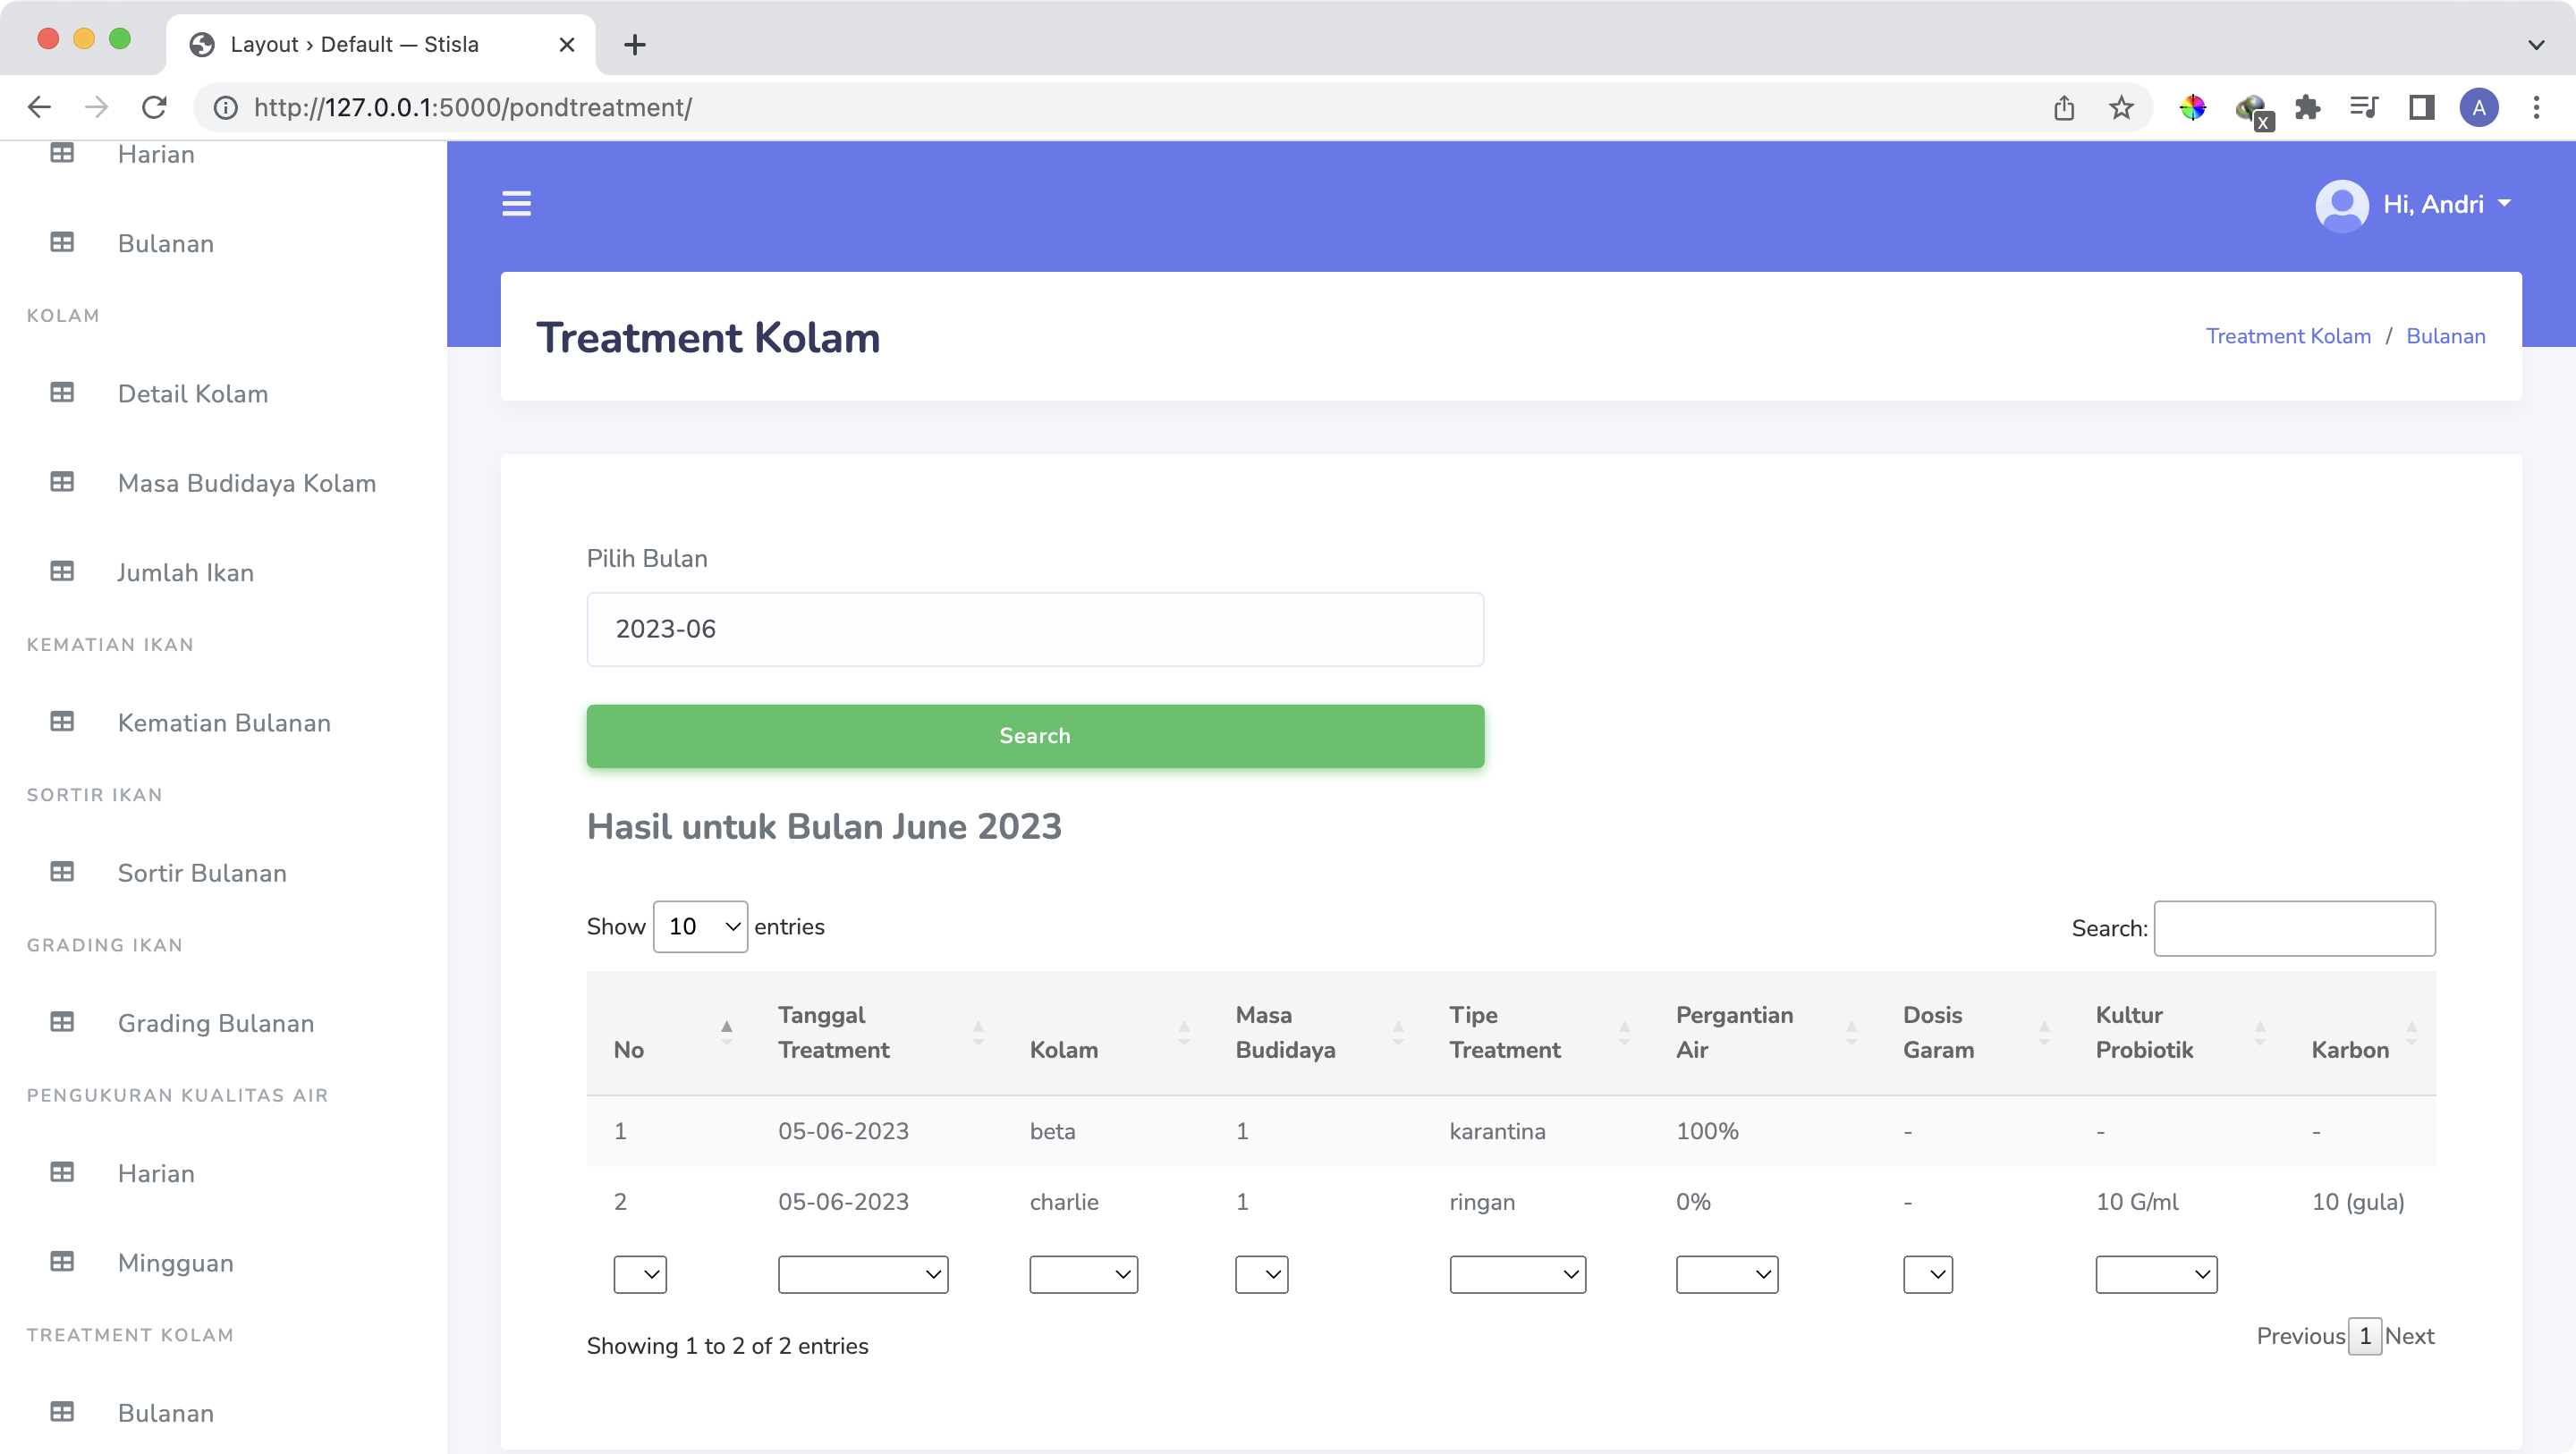
\includegraphics[width=1\textwidth]{gambar/Sprint10/view/view_rekap_treatment_kolam}
	\caption{View list pencatatan kolam harian}
	\label{fig:view_list_pencatatan_kolam_harian}
\end{figure}

\item \textbf{Membuat view rekap pencatatan kolam mingguan}
\begin{figure}[H]
	\centering
	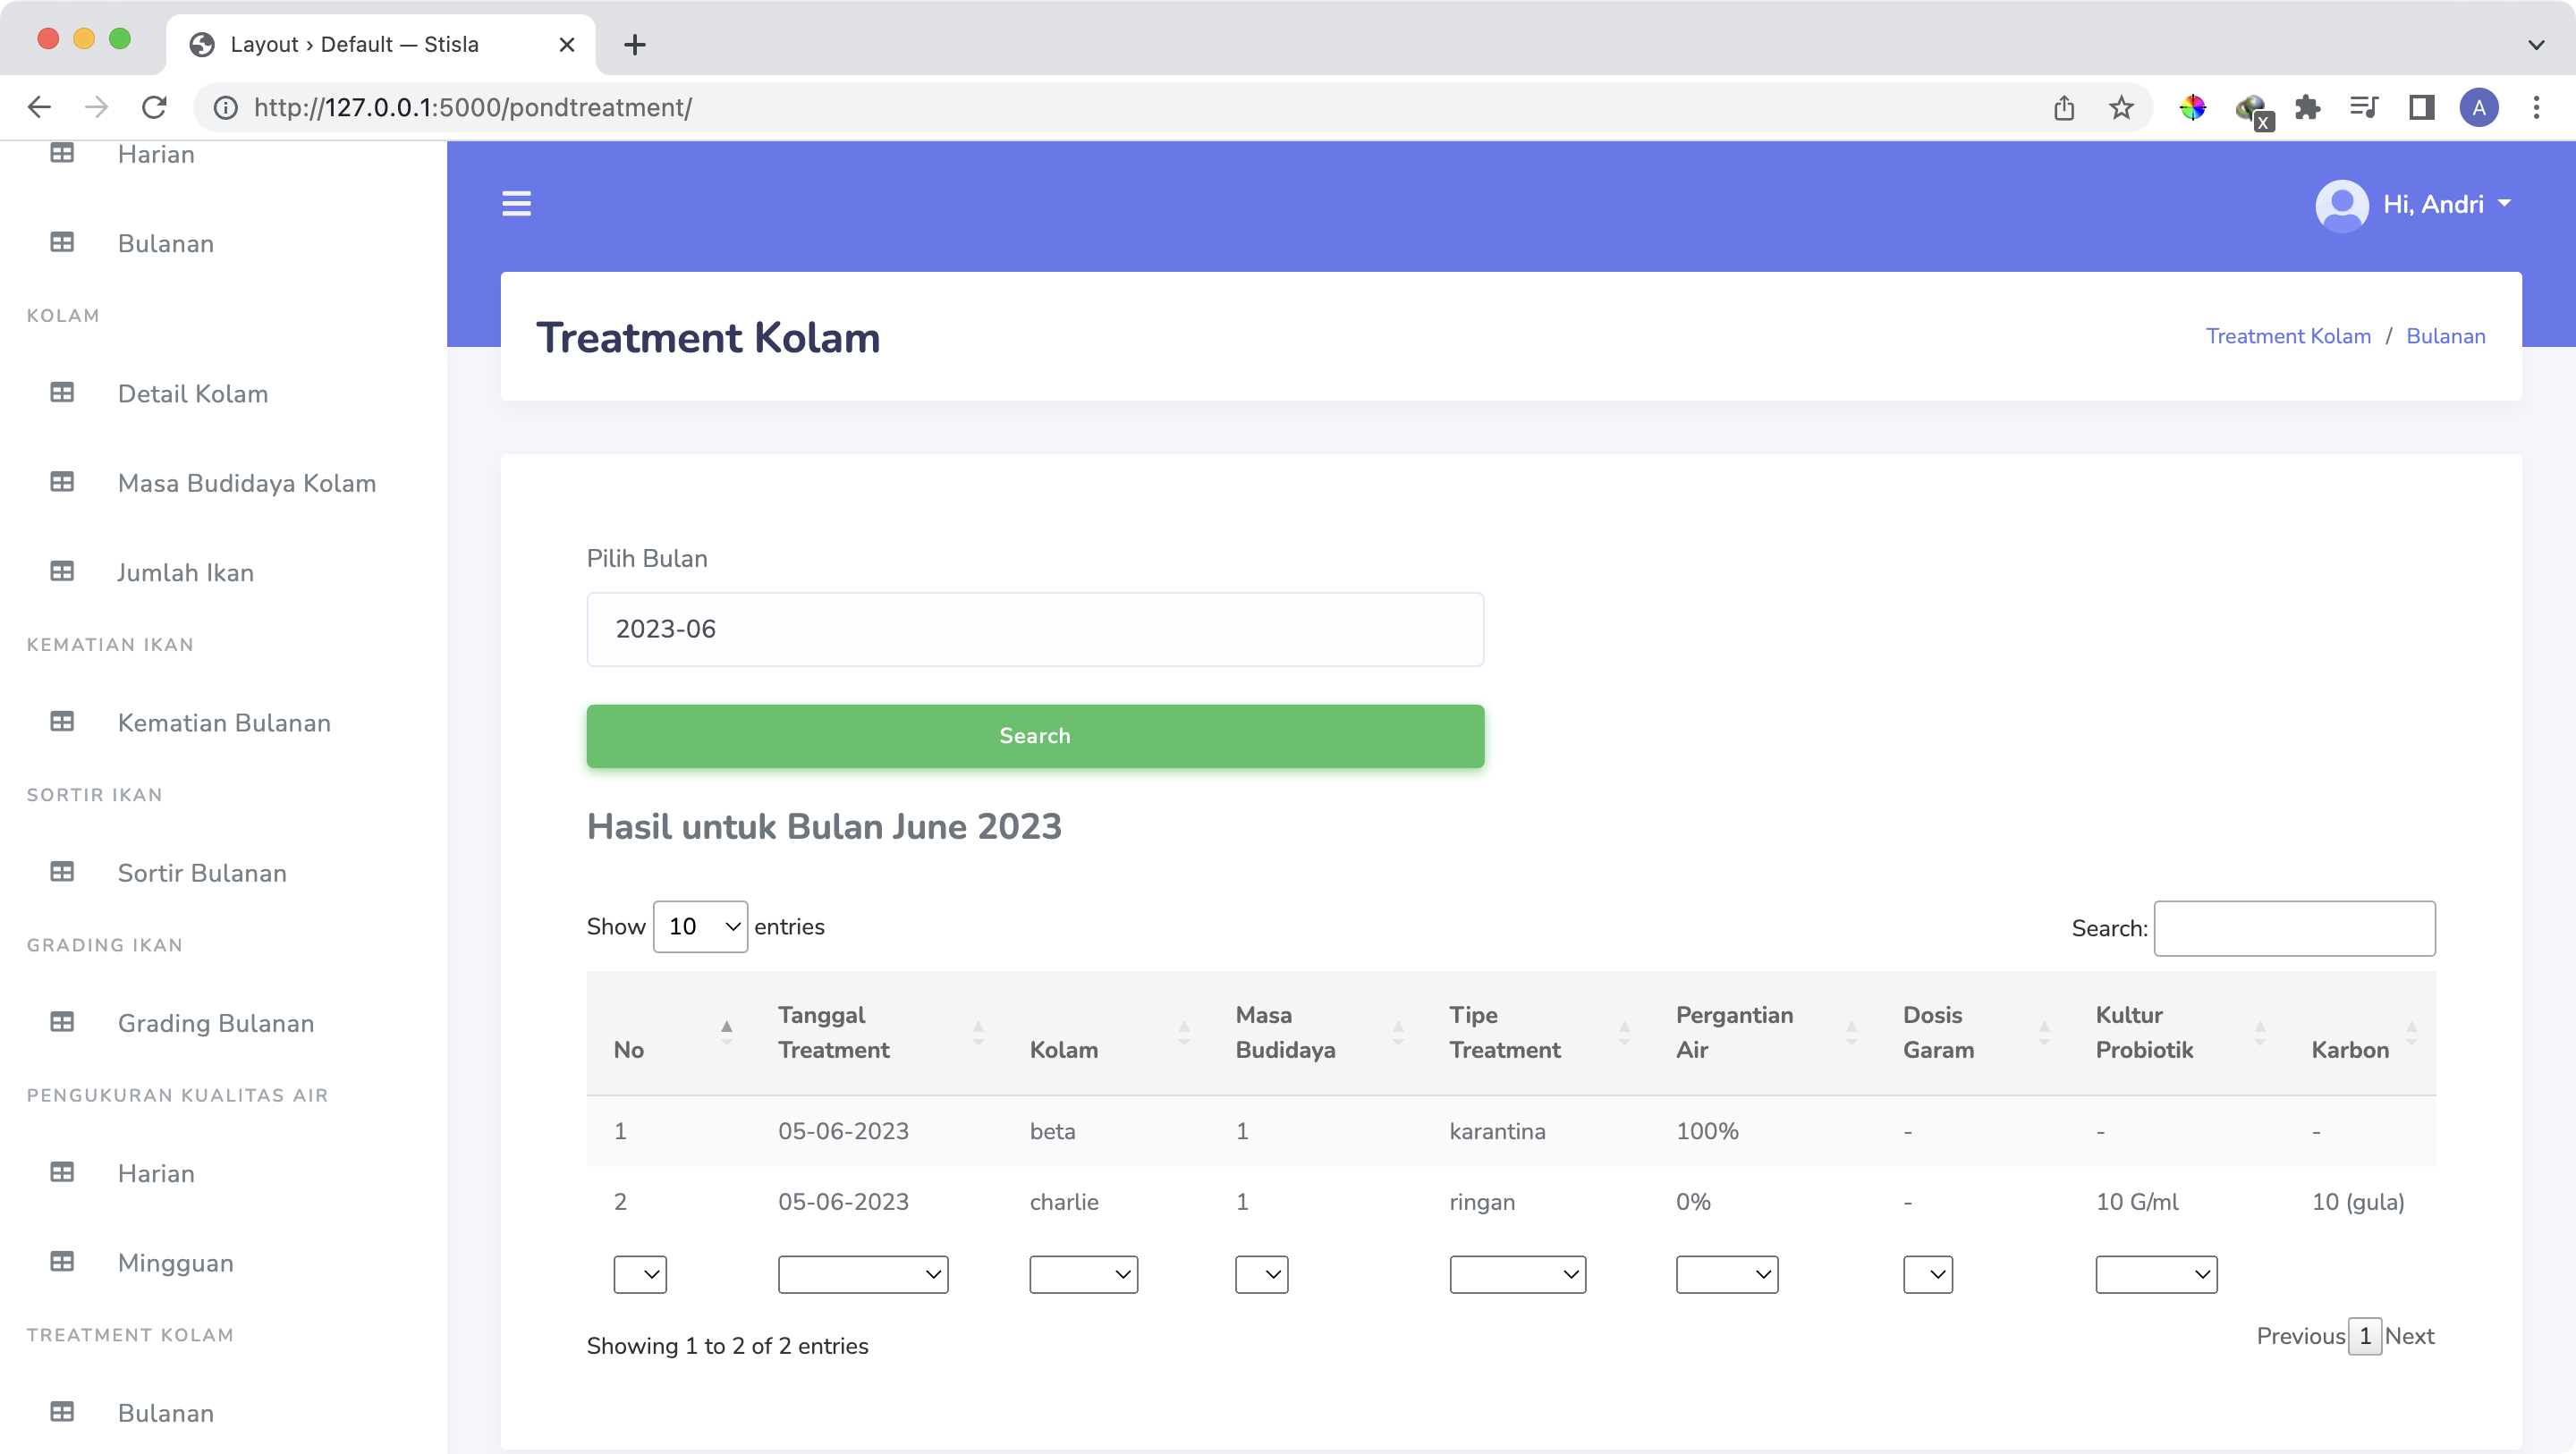
\includegraphics[width=1\textwidth]{gambar/Sprint10/view/view_rekap_treatment_kolam}
	\caption{View list pencatatan kolam mingguan}
	\label{fig:view_list_pencatatan_kolam_mingguan}
\end{figure}




\end{enumerate}